\chapter{Eikonal Coulomb Scattering\label{ChCoulomb}}
%%%%%%%%%%%%%%%%%%%%%%%%%%%%%%%%%%%%%%%%%%%%%%%%%%%%%%%%%%%%%%%%%%%%%%%%%%%%%%%%%%%%%%%%%
As an application of the nonrelativistic eikonal JWKB approximation, in this chapter we compute the four-point scattering amplitude for a two-body system of particles that are coupled to an instantaneous scalar wave field $U$. This system is analogous to two particles interacting via a Coulomb force. In principle, this problem is separable into two single-body problems. We will keep the ``two-body-ness'' explicit, as the methods we use will generalize to the relativistic theory. Coulomb scattering via the semiclassical eikonal approximation is treated (with less detail) in section 9.6.2 of \cite{ZinnJustin}. This problem is also considered in \cite{Glauber}.

We start with the two-body path integral,
\begin{equation}
	\mathcal{G}[U] = \int\limits_{\mathbf{x}_{1}}^{\mathbf{x}_{3}} \mathrm{D}\mathbf{q}_{a}(t) \int\limits_{\mathbf{x}_{2}}^{\mathbf{x}_{4}} \mathrm{D}\mathbf{q}_{b}(t) \, \exp{\left( - \frac{i}{\hbar} S_{P}[ \mathbf{q}_{a}, \mathbf{q}_{b}, U] \right)}
\end{equation}
This is a functional of the scalar wave field $U$. The particle action functional $S_{P}$ is
\begin{equation}
	S_{P}[ \mathbf{q}_{a}, \mathbf{q}_{b}, U] = S_{0}[ \mathbf{q}_{a}, \mathbf{q}_{b}] + S_{\text{int}}[ \mathbf{q}_{a}, \mathbf{q}_{b}, U]
\end{equation}
with the free term,
\begin{equation}
	S_{0}[ \mathbf{q}_{a}, \mathbf{q}_{b}] = \int \mathrm{d}t \left[ -\frac{m_{a}}{2} \dot{\mathbf{q}}_{a}^{2} - \frac{m_{b}}{2} \dot{\mathbf{q}}_{b}^{2} \right]
\end{equation}
and the term with the couplings to the field $U$,
\begin{equation}
	S_{\text{int}}[ \mathbf{q}_{a}, \mathbf{q}_{b}, U] = \int \mathrm{d}t \left( Z_{a} U[\mathbf{q}_{a}(t)] + Z_{b} U[\mathbf{q}_{b}(t)] \right) \label{SIntU}
\end{equation}
Here $Z_{a}$ and $Z_{b}$ are dimensionless charges for particles $a$ and $b$, respectively.

We integrate over the field $U$ to obtain the effective two-body quantum kernel:
\begin{equation}
	\mathcal{F}(3,4|1,2) \equiv \int \mathrm{D}U(\mathbf{x}) \, \mathcal{G}[U] \exp{\left(- \frac{i}{\hbar} S_{\text{kin}}[U] \right)} \label{FNR}
\end{equation}
Here, the functional $S_{\text{kin}}$ acts as a kinetic term for $U$,
\begin{equation}
	S_{\text{kin}}[U] = \frac{1}{2g^{2}} \int \int \mathrm{d}t_{x} \mathrm{d}t_{y} \int \int \mathrm{d}x \mathrm{d}y \left[ U(\mathbf{x}) K(\mathbf{x}, t_{x}| \mathbf{y}, t_{y}) U(\mathbf{y}) \right] \label{SKinU}
\end{equation}
where $K$ is the kinetic operator for an \textit{instantaneous} scalar wave,
\begin{equation}
	K(\mathbf{x}, t_{x}| \mathbf{y}, t_{y}) \equiv \delta(t_{x} - t_{y}) \delta(\mathbf{x} - \mathbf{y}) \left[ - \frac{1}{2} \left(\frac{\partial}{\partial \mathbf{x}} \right)^{2} \right]
\end{equation}
and $g$ is a dimensionful coupling parameter. The functional measure in (\ref{FNR}) is normalized such that
\begin{equation}
	\int \mathrm{D}U(\mathbf{x}) \, \exp{\left(- \frac{i}{\hbar} S_{\text{kin}}[U] \right)} = 1
\end{equation}
In the presence of $\mathcal{G}$, the functional integral over $U$ can be done exactly. Let
\begin{equation}
	J(\mathbf{x}, t) \equiv Z_{a} \delta[\mathbf{x} - \mathbf{q}_{a}(t)] + Z_{b} \delta[\mathbf{x} - \mathbf{q}_{b}(t)]
\end{equation}
such that we can rewrite $S_{\text{int}}$ as
\begin{equation}
	S_{\text{int}}[ \mathbf{q}_{a}, \mathbf{q}_{b}, U] = \int \mathrm{d} t \int \mathrm{d}x \, J(\mathbf{x}, t) U(\mathbf{x})
\end{equation}
After integration over $U$, one obtains
\begin{equation}
	\mathcal{F}(3,4|1,2) = \int\limits_{\mathbf{x}_{1}}^{\mathbf{x}_{3}} \mathrm{D}\mathbf{q}_{a}(t) \int\limits_{\mathbf{x}_{2}}^{\mathbf{x}_{4}} \mathrm{D}\mathbf{q}_{b}(t) \, \exp{\left( - \frac{i}{\hbar} S_{U}[ \mathbf{q}_{a}, \mathbf{q}_{b}] \right)} \label{FCoul}
\end{equation}
where the effective particle action functional $S_{U}$ is
\begin{equation}
\begin{split}
	S_{U}[q_{a}, q_{b}] = {}& S_{0}[ \mathbf{q}_{a}, \mathbf{q}_{b}] \\
	&- \frac{g^{2}}{2} \int \mathrm{d}t_{x} \mathrm{d}t_{y} \int \mathrm{d}x \mathrm{d}y \left[ J(\mathbf{x}, t_{x}) G(\mathbf{x}, t_{x}| \mathbf{y}, t_{y}) J(\mathbf{y}, t_{y}) \right]
\end{split}
\end{equation}
Here $G$ is the Green function for an \textit{instantaneous} scalar wave in $d$ spatial dimensions:
\begin{equation}
	G(\mathbf{x}, t_{x}| \mathbf{y}, t_{y}) = \delta(t_{x} - t_{y}) \Gamma\left( \frac{d - 2}{2} \right) \left( \frac{2}{(\mathbf{x} - \mathbf{y})^{2}} \right)^{(d - 2)/2}
\end{equation}
Using the explicit form of $J$, we find
\begin{equation}
	S_{U}[ \mathbf{q}_{a}, \mathbf{q}_{b}] = S_{0}[ \mathbf{q}_{a}, \mathbf{q}_{b}] - S_{1}[ \mathbf{q}_{a}, \mathbf{q}_{b} ] - S_{2}[ \mathbf{q}_{a}, \mathbf{q}_{b} ]
\end{equation}
where $S_{1}$ contains (divergent) one-body self-interactions and $S_{2}$ contains a two-body interaction. The contributions from the self-interactions are divergent because the require evaluating the Green function at the same spatial point. We will \textit{ignore} these contributions. Explicitly, $S_{2}$ is given by
\begin{equation}
	S_{2}[ \mathbf{q}_{a}, \mathbf{q}_{b} ] = g^{2} Z_{a} Z_{b} \Gamma\left( \frac{d - 2}{2} \right) \int \mathrm{d}t \left( \frac{2}{[\mathbf{q}_{a}(t) - \mathbf{q}_{b}(t)]^{2}} \right)^{(d - 2)/2}
\end{equation}
We have essentially derived the action functional for a two-body system of charged particles interacting via a Coulomb-like potential.

We now perform a little dimensional analysis. Note that we have kept $\hbar$ and the speed of light\footnote{Strictly speaking, the speed of light is infinite in the nonrelativistic theory.} dimensionful. All action functionals have units of $\hbar$. From (\ref{SIntU}) we find that the field $U$ has units of energy. Then, from (\ref{SKinU}) we find that the coupling parameter $g$ has units
\begin{equation}
	[g] = \frac{1}{2} [\hbar] + \frac{1}{2} [c] + \left( \frac{d - 3}{2} \right) [\text{length}]
\end{equation}
Thus, for $d = 3$ the coupling parameter $g$ has units
\begin{equation}
	[g] = \frac{1}{2} [\hbar] + \frac{1}{2} [c]
\end{equation}
We introduce a \textit{dimensionless} coupling parameter $\alpha$ via the equation
\begin{equation}
	g^{2} = \frac{\hbar c \alpha}{\sqrt{2 \pi}} L^{(3 - d)}
\end{equation}
where $L$ is a constant with units of length and the numerical factor in the denominator is for later convenience. Note that in $d = 3$ we recover the familiar dimensionless coupling, the fine-structure constant:
\begin{equation}
	\alpha \sim \frac{g^{2}}{\hbar c}
\end{equation}
If we keep $g^{2}$ fixed and take the limit $\hbar \rightarrow 0$ we find $\alpha \rightarrow \infty$. In other words, the semiclassical approximation is a \textit{strong-coupling} approximation. However, in the nonrelativistic theory we take the limit $c \rightarrow \infty$, which if we keep $g^{2}$ fixed leads us to $\alpha \rightarrow 0$. We will argue that, in principle, $\alpha$ is not well-defined in the nonrelativistic semiclassical theory. We will still use $\alpha$ (and $c$) as a formal symbol. This issue is not present in the semiclassical relativistic theory.
%%%%%%%%%%%%%%%%%%%%%%%%%%%%%%%%%%%%%%%%%%%%%%%%%%%%%%%%%%%%%%%%%%%%%%%%%%%%%%%%%%%%%%%%%
\section{Eikonal Kernel}
%%%%%%%%%%%%%%%%%%%%%%%%%%%%%%%%%%%%%%%%%%%%%%%%%%%%%%%%%%%%%%%%%%%%%%%%%%%%%%%%%%%%%%%%%
In the eikonal JWKB approximation, the quantum kernel (\ref{FCoul}) becomes the semiclassical eikonal kernel:
\begin{equation}
	\mathcal{F}(3,4|1,2) \longrightarrow \mathcal{E}(3,4|1,2) = \sqrt{\det{(\mathbf{V})}} \exp{\left( - \frac{i}{\hbar} \Sigma \right)}
\end{equation}
We have dropped the ``eik'' labels from the two-body eikonal Van Vleck function and the two-body eikonal Van Vleck matrix. The two-body eikonal Van Vleck function is
\begin{equation}
	\Sigma = S_{U}[ \mathbf{e}_{a}, \mathbf{e}_{b} ]
\end{equation}
and the two-body eikonal Van Vleck matrix is a $2 \times 2$ array of single-body eikonal Van Vleck matrices
\begin{equation}
	\mathbf{V} = \begin{pmatrix}
	\mathbf{V}_{13} & \mathbf{V}_{23} \\
	\mathbf{V}_{14} & \mathbf{V}_{24}
	\end{pmatrix}, \qquad \mathbf{V}_{jk} = - \frac{i}{\hbar} \frac{\partial^{2} \Sigma}{\partial \mathbf{x}_{j} \partial \mathbf{x}_{k}}
\end{equation}
In the two-body problem, the eikonal paths are
\begin{equation}
\begin{split}
	\mathbf{e}_{a}(t) &= \frac{\mathbf{x}_{1} + \mathbf{x}_{3}}{2} + \left( \mathbf{x}_{3} - \mathbf{x}_{1} \right) \left( \frac{t}{\Delta t} \right) \\
	\mathbf{e}_{b}(t) &= \frac{\mathbf{x}_{2} + \mathbf{x}_{4}}{2} + \left( \mathbf{x}_{4} - \mathbf{x}_{2} \right) \left( \frac{t}{\Delta t} \right)
\end{split} \label{NReikPath}
\end{equation}
For convenience, the range of the time parameter $t$ is
\begin{equation}
	{ -\frac{\Delta t}{2} } < t < \frac{\Delta t}{2}, \qquad \Delta t = t_{O} - t_{I} > 0
\end{equation}
We now determine $\Sigma$ and $\mathbf{V}$.
%%%%%%%%%%%%%%%%%%%%%%%%%%%%%%%%%%%%%%%%%%%%%%%%%%%%%%%%%%%%%%%%%%%%%%%%%%%%%%%%%%%%%%%%%
\subsection{Eikonal Van Vleck Function}
%%%%%%%%%%%%%%%%%%%%%%%%%%%%%%%%%%%%%%%%%%%%%%%%%%%%%%%%%%%%%%%%%%%%%%%%%%%%%%%%%%%%%%%%%
At the eikonal paths (\ref{NReikPath}), the free term in the action functional becomes
\begin{align}
	\Sigma_{0} &\equiv S_{0}\left[ \mathbf{e}_{a}, \mathbf{e}_{b} \right] \nonumber \\
	&= -\frac{m_{a}}{2 \Delta t} \left( \mathbf{x}_{3} - \mathbf{x}_{1} \right)^{2} - \frac{m_{b}}{2 \Delta t} \left( \mathbf{x}_{4} - \mathbf{x}_{2} \right)^{2} \label{Sigma0NR}
\end{align}
Similarly, the two-body interaction term becomes
\begin{align}
	\Sigma_{2} &\equiv S_{2}\left[ \mathbf{e}_{a}, \mathbf{e}_{b} \right] \nonumber \\
	&= g^{2} Z_{a} Z_{b} \Gamma\left( \frac{d - 2}{2} \right) \int \mathrm{d}t \left( \frac{2}{[\mathbf{e}_{a}(t) - \mathbf{e}_{b}(t)]^{2}} \right)^{(d - 2)/2} \label{Sigma2NR}
\end{align}
With the eikonal paths (\ref{NReikPath}), we have
\begin{equation}
	\mathbf{e}_{a}(t) - \mathbf{e}_{b}(t) = \mathbf{X} - \mathbf{x} \left( \frac{t}{\Delta t} \right)
\end{equation}
and thus
\begin{equation}
	[\mathbf{e}_{a}(t) - \mathbf{e}_{b}(t)]^{2} = \mathbf{X}^{2} - 2 (\mathbf{X} \cdot \mathbf{x}) \left( \frac{t}{\Delta t} \right) + \mathbf{x}^{2} \left( \frac{t}{\Delta t} \right)^{2}
\end{equation}
where we have introduced the vectors
\begin{equation}
	\mathbf{X} \equiv \frac{\mathbf{x}_{1} - \mathbf{x}_{2} + \mathbf{x}_{3} - \mathbf{x}_{4}}{2} , \qquad \mathbf{x} \equiv \mathbf{x}_{4} - \mathbf{x}_{2} - \mathbf{x}_{3} + \mathbf{x}_{1}
\end{equation}
The vector $\mathbf{X}$ corresponds to the \textit{vector average} of the initial separation of the particles (given by $\mathbf{x}_{1} - \mathbf{x}_{2}$) and the final separation (given by $\mathbf{x}_{3} - \mathbf{x}_{4}$).

%We will first evaluate the time integral in (\ref{Sigma2NR}) exactly (i.e. ignoring the eikonal JWKB approximation). Let
%\begin{equation}
%	u \equiv \frac{t}{\Delta t}
%\end{equation}
%Then
%\begin{equation}
%	{ - \frac{\Delta t}{2} } < t < \frac{\Delta t}{2} \Longrightarrow { - \frac{1}{2} } < u < \frac{1}{2}, \qquad \mathrm{d}t = \Delta t \mathrm{d}u
%\end{equation}
%We introduce dimensionless variables $r$ and $\beta$,
%\begin{equation}
%	r \equiv \frac{|\mathbf{x}|}{|\mathbf{X}|}, \qquad \beta \equiv \frac{\mathbf{X} \cdot \mathbf{x}}{|\mathbf{X}| |\mathbf{x}|}
%\end{equation}
%Note that
%\begin{equation}
%	r > 0, \qquad {-1} < \beta < 1
%\end{equation}
%In terms of these variables, we have
%\begin{equation}
%	[\mathbf{e}_{a}(t) - \mathbf{e}_{b}(t)]^{2} = \mathbf{X}^{2} \left[1 - 2 \beta r u + r^{2} u^{2} \right]
%\end{equation}
%Next we introduce
%\begin{equation}
%	v \equiv r u
%\end{equation}
%with
%\begin{equation}
%	{ - \frac{1}{2} } < u < \frac{1}{2} \Longrightarrow { - \frac{r}{2} } < v < \frac{r}{2}, \qquad \mathrm{d}t = \frac{\Delta t}{r} \mathrm{d}v
%\end{equation}
%So we write
%\begin{align}
%	[\mathbf{e}_{a}(t) - \mathbf{e}_{b}(t)]^{2} &= \mathbf{X}^{2} \left[1 - 2 \beta v + v^{2} \right] \nonumber \\
%	&= \mathbf{X}^{2} \left[1 - \beta^{2} + (v - \beta)^{2} \right]
%\end{align}
%Finally, we introduce
%\begin{equation}
%	w \equiv \frac{v - \beta}{\sqrt{1 - \beta^{2}}}
%\end{equation}
%with
%\begin{equation}
%	{- \frac{r + 2 \beta}{2\sqrt{1 - \beta^{2}}} } < w < \frac{r - 2 \beta}{2\sqrt{1 - \beta^{2}}}, \qquad \mathrm{d}t = \frac{\Delta t \sqrt{1 - \beta^{2}}}{r} \mathrm{d}w
%\end{equation}
%We can finally write
%\begin{equation}
%	[\mathbf{e}_{a}(t) - \mathbf{e}_{b}(t)]^{2} = \mathbf{X}^{2} \left( 1 - \beta^{2} \right) \left(1 + w^{2} \right)
%\end{equation}
%In $d = 3$, we have
%\begin{align}
%	\Sigma_{2} &= \hbar \alpha \left( \frac{Z_{a} Z_{b} c \Delta t}{|\mathbf{x}|} \right) \left[ \int \mathrm{d}w \frac{1}{\sqrt{1 + w^{2}}} \right] \nonumber \\
%	&= \hbar \alpha \left( \frac{Z_{a} Z_{b} c \Delta t}{|\mathbf{x}|} \right) \left[ \operatorname{arcsinh}{(w_{O})} - \operatorname{arcsinh}{(w_{I})} \right]
%\end{align}
%with
%\begin{equation}
%	w_{I} = - \frac{r + 2 \beta}{2\sqrt{1 - \beta^{2}}}, \qquad w_{O} = \frac{r - 2 \beta}{2\sqrt{1 - \beta^{2}}}
%\end{equation}
%We now decompose the vector $\mathbf{X}$ into the component parallel to $\mathbf{x}$ and the component orthogonal to $\mathbf{x}$:
%\begin{equation}
%	\mathbf{X} = \mathbf{B} + b\mathbf{x}, \qquad \mathbf{B} \cdot \mathbf{x} = 0
%\end{equation}
%That is,
%\begin{equation}
%	b = \frac{\mathbf{X} \cdot \mathbf{x}}{\mathbf{x}^{2}}, \qquad \mathbf{B} = \mathbf{X} - \left( \frac{\mathbf{X} \cdot \mathbf{x}}{\mathbf{x}^{2}} \right) \mathbf{x}
%\end{equation}
%In terms of $r$ and $\beta$ we have
%\begin{equation}
%	b = \frac{\beta}{r}, \qquad |\mathbf{B}| = |\mathbf{X}| \sqrt{1 - \beta^{2}}
%\end{equation}
%Thus,
%\begin{equation}
%	w_{I} = - \frac{|\mathbf{x}|}{2 |\mathbf{B}|} \left(1 + 2 b \right), \qquad w_{O} = \frac{|\mathbf{x}|}{2 |\mathbf{B}|} \left(1 - 2 b \right)
%\end{equation}
%Recall that
%\begin{equation}
%	\operatorname{arcsinh}{(x)} = \log{\left( \sqrt{1 + x^{2}} + x \right)}
%	%= \log{\left( \frac{1}{\sqrt{1 + x^{2}} - x} \right)}
%\end{equation}
%Hence
%\begin{align}
%	\operatorname{arcsinh}{(w_{O})} &= \log{\left( \frac{|\mathbf{x}|}{2 |\mathbf{B}|} \left(1 - 2 b \right) + \sqrt{1 + \frac{\mathbf{x}^{2}}{4 \mathbf{B}^{2}} \left(1 - 2 b \right)^{2}} \right)} \\
%	{- \operatorname{arcsinh}{(w_{I})}} &= \log{\left( \frac{|\mathbf{x}|}{2 |\mathbf{B}|} \left(1 + 2 b \right) + \sqrt{1 + \frac{\mathbf{x}^{2}}{4 \mathbf{B}^{2}} \left(1 + 2 b \right)^{2}} \right)}
%\end{align}
%Integrate over x with stationary methods, then there will be Delta t dependence inside the log. This is dangerous when taking the large time interval limit. So the infrared divergence reappears.

In order to evaluate the integral over $t$ in (\ref{Sigma2NR}), we first introduce a Schwinger variable $\omega$ and write
\begin{equation}
	\Sigma_{2} = \frac{\hbar c \alpha Z_{a} Z_{b} L}{\sqrt{2 \pi}} \int\limits_{0}^{\infty}\mathrm{d}\omega \left( \frac{1}{\omega} \right)^{d/2} \int \mathrm{d}t \, \exp{\left( - \frac{1}{2 \omega L^{2}} [\mathbf{e}_{a}(t) - \mathbf{e}_{b}(t)]^{2} \right)}
\end{equation}
This way, the integrand becomes a Gaussian. In the eikonal approximation, the momentum transfer between the particles is small when compared to other momenta in the problem. The Fourier-Heisenberg conjugate of this statement is that the separation between the particles is always large when compared to other distances in the problem. Thus,
\begin{equation}
	\frac{1}{2 L^{2}} [\mathbf{e}_{a}(t) - \mathbf{e}_{b}(t)]^{2} \gg 1
\end{equation}
In this regime, the integral over $t$ can be evaluated with stationary methods. The stationary point is
\begin{equation}
	t_{*} = \Delta t \left( \frac{\mathbf{X} \cdot \mathbf{x}}{\mathbf{x}^{2}} \right)
\end{equation}
This value of the time parameter yields the minimum separation between the particles,
\begin{equation}
	\mathbf{B} \equiv \mathbf{e}_{a}(t_{*}) - \mathbf{e}_{b}(t_{*}) = \mathbf{X} - \left( \frac{\mathbf{X} \cdot \mathbf{x}}{\mathbf{x}^{2}} \right) \mathbf{x}
\end{equation}
as long as
\begin{equation}
	{- \frac{1}{2}} < \frac{\mathbf{X} \cdot \mathbf{x}}{\mathbf{x}^{2}} < \frac{1}{2}
\end{equation}
Note that the vector $\mathbf{B}$ is orthogonal to $\mathbf{x}$, so it only has $d - 1$ independent components.

After dealing with the integration over $t$, we find
\begin{equation}
	\Sigma_{2} \approx \hbar \alpha \left[ \frac{Z_{a} Z_{b} c \Delta t}{|\mathbf{x}|} \right] \int\limits_{0}^{\infty}\mathrm{d}\omega \left( \frac{1}{\omega} \right)^{(d - 1)/2} \exp{\left( - \frac{1}{2 \omega L^{2}} \mathbf{B}^{2} \right)}
\end{equation}
which, after integration over $\omega$, yields
\begin{equation}
	\Sigma_{2} \approx \hbar \alpha \left[ \frac{Z_{a} Z_{b} c \Delta t}{|\mathbf{x}|} \right] \Gamma\left( \frac{d - 3}{2} \right) \left( \frac{2 L^{2}}{\mathbf{B}^{2}} \right)^{(d - 3) / 2}
\end{equation}
This result is divergent in $d = 3$, which happens to be the case of most relevance. We will use dimensional regularization by setting $d = 3 + 2 \varepsilon$ with $\varepsilon > 0$. After introducing
\begin{equation}
	\rho \equiv \frac{Z_{a} Z_{b} c \Delta t}{|\mathbf{x}|}
\end{equation}
we can write
\begin{equation}
	\Sigma_{2} \approx \hbar \alpha \rho \Gamma(\varepsilon) \left( \frac{2 L^{2}}{\mathbf{B}^{2}} \right)^{\varepsilon} \label{Sigma2NR2}
\end{equation}
We will find similar expressions in the relativistic theory.

The divergence in $\Sigma_{2}$ is somewhat troubling. One could think that this divergence follows as a consequence of using stationary methods for evaluating the integral over $t$. In principle, we can evaluate the integral over $t$ in $d = 3$ exactly and obtain a result that does not exhibit explicit divergences. However, when we use the resulting semiclassical eikonal kernel to obtain the asymptotic S-matrix, we need to take the large $\Delta t$ limit. The result from the exact integral is divergent in this limit, so a divergence is re-introduced into the problem (similar issues are encountered in \cite{ZinnJustin}). Our result (\ref{Sigma2NR2}) has an implicit $\Delta t$ hidden in $\rho$, but we will see that the particular combination in $\rho$ is finite.
%%%%%%%%%%%%%%%%%%%%%%%%%%%%%%%%%%%%%%%%%%%%%%%%%%%%%%%%%%%%%%%%%%%%%%%%%%%%%%%%%%%%%%%%%
\subsection{Eikonal Van Vleck Matrix}
%%%%%%%%%%%%%%%%%%%%%%%%%%%%%%%%%%%%%%%%%%%%%%%%%%%%%%%%%%%%%%%%%%%%%%%%%%%%%%%%%%%%%%%%%
The two-body eikonal Van Vleck matrix has four blocks:
\begin{equation}
	\mathbf{V} = \begin{pmatrix}
	\mathbf{V}_{13} & \mathbf{V}_{23} \\
	\mathbf{V}_{14} & \mathbf{V}_{24}
	\end{pmatrix}, \qquad \mathbf{V}_{jk} = - \frac{i}{\hbar} \frac{\partial^{2} \Sigma}{\partial \mathbf{x}_{j} \partial \mathbf{x}_{k}}
\end{equation}
Since $\Sigma$ has the form $\Sigma_{0} - \Sigma_{2}$, we write
\begin{equation}
	\mathbf{V} = \mathbf{V}_{0} - \mathbf{V}_{2} = \left(\mathbf{I} - \mathbf{W} \right) \cdot \mathbf{V}_{0}, \qquad \mathbf{W} \equiv \mathbf{V}_{2} \cdot (\mathbf{V}_{0})^{-1}
\end{equation}
Taking the determinant gives
\begin{equation}
	\det{(\mathbf{V})} = \det{(\mathbf{I} - \mathbf{W})} \det{(\mathbf{V}_{0})}
\end{equation}
Now, recall the identity
\begin{equation}
	\det{(\mathbf{I} - \mathbf{W})} = \exp{\left[- \sum_{n = 1}^{\infty} \frac{1}{n} \operatorname{tr}{(\mathbf{W}^{n})} \right]}
\end{equation}
Thus,
\begin{equation}
	\sqrt{\det{(\mathbf{V})}} = \sqrt{\det{(\mathbf{V}_{0})}} \exp{\left[- \frac{1}{2} \sum_{n = 1}^{\infty} \frac{1}{n} \operatorname{tr}{(\mathbf{W}^{n})} \right]}
\end{equation}

The free part $\mathbf{V}_{0}$ is easy to obtain. We have
\begin{equation}
	\mathbf{V}_{0} = \begin{pmatrix}
	\mathbf{u}_{13} & \mathbf{u}_{23} \\
	\mathbf{u}_{14} & \mathbf{u}_{24}
	\end{pmatrix}, \qquad \mathbf{u}_{jk} = - \frac{i}{\hbar} \frac{\partial^{2} \Sigma_{0}}{\partial \mathbf{x}_{j} \partial \mathbf{x}_{k}}
\end{equation}
With (\ref{Sigma0NR}), we find
\begin{equation}
\begin{split}
	\mathbf{u}_{13} = \left(- \frac{i m_{a}}{\hbar \Delta t} \right) \mathbf{I}, \qquad \mathbf{u}_{23} = \mathbf{u}_{14} = \mathbf{0}, \qquad \mathbf{u}_{24} = \left(- \frac{i m_{b}}{\hbar \Delta t} \right) \mathbf{I}
\end{split}
\end{equation}
Hence, $\mathbf{V}_{0}$ is invertible and thus $\mathbf{W}$ is well-defined. However, as part of our approximations, we will neglect all the contributions to the determinant from $\mathbf{W}$. In principle, these contributions are very interesting, since they involve the coupling parameter $\alpha$. In practice, all of these contributions are subleading in powers of $\mathbf{B}^{2}$, and we only keep the leading contribution that comes from $\Sigma_{2}$. Note that the determinant of $\mathbf{V}$ corresponds to the order-zero in $\hbar$ correction to the Van Vleck function. We have found that this $\hbar$-correction is nonperturbative in $\alpha$ since it involves an infinite number of contributions (coming from $\mathbf{W}$). This is a nice example of how the semiclassical approximation is nonperturbative.
%%%%%%%%%%%%%%%%%%%%%%%%%%%%%%%%%%%%%%%%%%%%%%%%%%%%%%%%%%%%%%%%%%%%%%%%%%%%%%%%%%%%%%%%%
\section{Semiclassical Eikonal S-Matrix}
%%%%%%%%%%%%%%%%%%%%%%%%%%%%%%%%%%%%%%%%%%%%%%%%%%%%%%%%%%%%%%%%%%%%%%%%%%%%%%%%%%%%%%%%%
With $\Sigma$ and $\mathbf{V}$ we can build the semiclassical eikonal kernel:
\begin{equation}
	\mathcal{E}(3,4|1,2) = \left(- \frac{i m_{a}}{\hbar \Delta t} \right)^{d/2} \left(- \frac{i m_{b}}{\hbar \Delta t} \right)^{d/2} \exp{\left(- \frac{i}{\hbar} \Sigma_{0} + \frac{i}{\hbar} \Sigma_{2} \right)}
\end{equation}
%where we have subtracted the disconnected part. We can write
%\begin{equation}
%	{-1} + \exp{\left( \frac{i}{\hbar} \Sigma_{2} \right)} = \sum_{l = 1}^{\infty} \frac{(i\alpha \rho)^{l}}{\Gamma(l+1)} [\Gamma(\varepsilon)]^{l} \left( \frac{2 L^{2}}{\mathbf{B}^{2}} \right)^{l \varepsilon}
%\end{equation}
We are interested in the three-dimensional theory, so we expand near $\varepsilon = 0$:
\begin{equation}
	\frac{i}{\hbar} \Sigma_{2} \approx i \alpha \rho \left[ \Gamma(\varepsilon) + \log{\left( \frac{2 L^{2}}{\mathbf{B}^{2}} \right)} \right]
\end{equation}
Thus
\begin{equation}
	\exp{\left( \frac{i}{\hbar} \Sigma_{2} \right)} \approx \left( \frac{2 L^{2}}{\mathbf{B}^{2}} \right)^{i \alpha \rho} \exp{\left( \Lambda_{\varepsilon} \right)}
\end{equation}
with
\begin{equation}
	\Lambda_{\varepsilon} \equiv i \alpha \rho \Gamma(\varepsilon)
\end{equation}

The semiclassical eikonal S-matrix is
\begin{equation}
	\mathcal{S}(3,4|1,2) = \int \int \int \int \mathrm{d}x_{1} \mathrm{d}x_{2} \mathrm{d}x_{3} \mathrm{d}x_{4} \, \overline{\mathcal{U}}_{O}(3,4) \mathcal{U}_{I}(1,2) \mathcal{E}(3,4|1,2)
\end{equation}
where
\begin{align}
	\mathcal{U}_{I}(1,2) &= \exp{\left[ \frac{i}{\hbar} \left( \mathbf{x}_{1} \cdot \mathbf{p}_{1} + \mathbf{x}_{2} \cdot \mathbf{p}_{2} \right) - \frac{i t_{I}}{\hbar} \left( \frac{\mathbf{p}_{1}^{2}}{2 m_{a}} + \frac{\mathbf{p}_{2}^{2}}{2 m_{b}} \right) \right]} \\
	\overline{\mathcal{U}}_{O}(3,4) &= \exp{\left[ -\frac{i}{\hbar} \left( \mathbf{x}_{3} \cdot \mathbf{p}_{3} + \mathbf{x}_{4} \cdot \mathbf{p}_{4} \right) + \frac{i t_{O}}{\hbar} \left( \frac{\mathbf{p}_{3}^{2}}{2 m_{a}} + \frac{\mathbf{p}_{4}^{2}}{2 m_{b}} \right) \right]}
\end{align}
With $\mathcal{S}$, we compute the asymptotic semiclassical eikonal S-matrix:
\begin{equation}
	\mathcal{A}(3,4|1,2) = \left[ \lim_{T \rightarrow \infty} \right] \left[ \lim_{t_{O} \rightarrow + T/2} \right] \left[ \lim_{t_{I} \rightarrow - T/2} \right] \mathcal{S}(3,4|1,2)
\end{equation}
We will apply these three limits in two stages. First, we apply the last two limits: these just set $t_{I} = -T/2$ and $t_{F} = T/2$. Hence,
\begin{equation}
	\Delta t = t_{F} - t_{I} = T 
\end{equation}
The third limit will be taken later.

In order to perform the integration to obtain $\mathcal{S}$ we first make a change of variables in the position basis and introduce the corresponding conjugate momenta:
\begin{equation}
\begin{split}
	\mathbf{R} \equiv \frac{\mathbf{x}_{1} + \mathbf{x}_{2} + \mathbf{x}_{3} + \mathbf{x}_{4}}{4} &\qquad \mathbf{K} \equiv \mathbf{p}_{4} + \mathbf{p}_{3} - \mathbf{p}_{2} - \mathbf{p}_{1} \\
	\mathbf{X} \equiv \frac{\mathbf{x}_{1} - \mathbf{x}_{2} + \mathbf{x}_{3} - \mathbf{x}_{4}}{2} &\qquad \mathbf{P} \equiv \frac{\mathbf{p}_{3} - \mathbf{p}_{1} + \mathbf{p}_{2} - \mathbf{p}_{4}}{2} \\
	\mathbf{x}_{31} \equiv \mathbf{x}_{3} - \mathbf{x}_{1} &\qquad \mathbf{p}_{31} \equiv \frac{\mathbf{p}_{1} + \mathbf{p}_{3}}{2} \\
	\mathbf{x}_{42} \equiv \mathbf{x}_{4} - \mathbf{x}_{2} &\qquad \mathbf{p}_{42} \equiv \frac{\mathbf{p}_{2} + \mathbf{p}_{4}}{2}
\end{split}
\end{equation}
such that
\begin{equation}
	\mathbf{x}_{1} \cdot \mathbf{p}_{1} + \mathbf{x}_{2} \cdot \mathbf{p}_{2} - \mathbf{x}_{3} \cdot \mathbf{p}_{3} - \mathbf{x}_{4} \cdot \mathbf{p}_{4} = - \mathbf{R} \cdot \mathbf{K} - \mathbf{X} \cdot \mathbf{P} - \mathbf{x}_{31} \cdot \mathbf{p}_{31} - \mathbf{x}_{42} \cdot \mathbf{p}_{42}
\end{equation}
Note that
\begin{equation}
	\mathbf{p}_{1}^{2} + \mathbf{p}_{3}^{2} = \frac{1}{8} \left( \mathbf{K} + 2 \mathbf{P} \right)^{2} + 2 \mathbf{p}_{31}^{2}
\end{equation}
and
\begin{equation}
	\mathbf{p}_{2}^{2} + \mathbf{p}_{4}^{2} = \frac{1}{8} \left( \mathbf{K} - 2 \mathbf{P} \right)^{2} + 2 \mathbf{p}_{42}^{2}
\end{equation}
These two identities allow us to write
\begin{equation}
\begin{split}
	\overline{\mathcal{U}}_{O} \mathcal{U}_{I} = {}& \exp{\left[ -\frac{i}{\hbar} \mathbf{x}_{31} \cdot \mathbf{p}_{31} - \frac{i}{\hbar} \mathbf{x}_{42} \cdot \mathbf{p}_{42} - \frac{i}{\hbar} \left( \mathbf{R} \cdot \mathbf{K} + \mathbf{X} \cdot \mathbf{P} \right) \right]} \\
	&\times \exp{\left( \frac{i T}{2 m_{a} \hbar} \mathbf{p}_{31}^{2} + \frac{i T}{2 m_{b} \hbar} \mathbf{p}_{42}^{2} \right)} \\
	&\times \exp{\left( \frac{i T}{8 \hbar} \left[ \frac{1}{4m_{a}} \left( \mathbf{K} + 2 \mathbf{P} \right)^{2} + \frac{1}{4m_{b}} \left( \mathbf{K} - 2 \mathbf{P} \right)^{2} \right] \right)}
\end{split} \label{thirdLine}
\end{equation}
Since $\mathcal{E}$ has no dependence on $\mathbf{R}$, the integral yields a Dirac delta:
\begin{equation}
	\int \mathrm{d}R \, \exp{\left(- \frac{i}{\hbar} \mathbf{R} \cdot \mathbf{K} \right)} = \hbar^{d} \delta(\mathbf{K})
\end{equation}
This Dirac delta imposes the constraint $\mathbf{K} = 0$ which leads to
\begin{equation}
	\mathbf{p}_{1} + \mathbf{p}_{2} = \mathbf{p}_{3} + \mathbf{p}_{4}
\end{equation}
This is nothing more than the conservation of the total external momentum. After this constraint is enforced, we have
\begin{equation}
	\mathbf{P} = \mathbf{p}_{3} - \mathbf{p}_{1} = \mathbf{p}_{2} - \mathbf{p}_{4}
\end{equation}
That is, $\mathbf{P}$ measures the momentum transfer between the particles. The eikonal paths (\ref{NReikPath}) are valid in the regime where the incoming and outgoing momenta of each particle is much larger than the momentum transfer between the particles. That is,
\begin{equation}
	\mathbf{p}_{1}^{2} \gg \mathbf{P}^{2} \qquad \mathbf{p}_{2}^{2} \gg \mathbf{P}^{2} \qquad \mathbf{p}_{3}^{2} \gg \mathbf{P}^{2} \qquad \mathbf{p}_{4}^{2} \gg \mathbf{P}^{2}
\end{equation}
It then follows that
\begin{equation}
	\mathbf{p}_{31}^{2} \gg \mathbf{P}^{2} \qquad \mathbf{p}_{42}^{2} \gg \mathbf{P}^{2}
\end{equation}
This argument enables us to neglect the third line in (\ref{thirdLine}). Thus, after the integration over $\mathbf{R}$ and using the eikonal approximation, we obtain
\begin{equation}
\begin{split}
	\overline{\mathcal{U}}_{O}(3,4) \mathcal{U}_{I}(1,2) = {}& \exp{\left[ -\frac{i}{\hbar} \mathbf{x}_{31} \cdot \mathbf{p}_{31} - \frac{i}{\hbar} \mathbf{x}_{42} \cdot \mathbf{p}_{42} - \frac{i}{\hbar} \mathbf{X} \cdot \mathbf{P} \right]} \\
	&\times \exp{\left[ \frac{i T}{2 m_{a} \hbar} \mathbf{p}_{31}^{2} + \frac{i T}{2 m_{b} \hbar} \mathbf{p}_{42}^{2} \right]}
\end{split}
\end{equation}

Next, we tackle the integration over $\mathbf{x}_{31}$ and $\mathbf{x}_{42}$. The exact integration is nontrivial since $\rho$ is a function of $\mathbf{x} = \mathbf{x}_{42} - \mathbf{x}_{31}$. We make another change of variables:
\begin{equation}
	\mathbf{x}_{31} = \frac{T}{m_{a}} \mathbf{k}_{31}, \qquad \mathbf{x}_{42} = \frac{T}{m_{b}} \mathbf{k}_{42}
\end{equation}
Then
\begin{equation}
	\frac{\mathbf{x}}{c T} = \frac{\mathbf{k}_{42}}{m_{b}c} - \frac{\mathbf{k}_{31}}{m_{a}c} = \left( \frac{m_{a} + m_{b}}{m_{a} m_{b} c} \right) \left( \frac{m_{a} \mathbf{k}_{24} - m_{b} \mathbf{k}_{31}}{m_{a} + m_{b}} \right) \equiv \frac{\mathbf{k}}{m c}
\end{equation}
where $m$ is the reduced mass,
\begin{equation}
	m \equiv \frac{m_{a} m_{b}}{m_{a} + m_{b}}
\end{equation}
Thus, $\rho$ has no explicit dependence on $T$ when written in terms of $\mathbf{k}_{31}$ and $\mathbf{k}_{42}$. We now have
\begin{equation}
\begin{split}
	\overline{\mathcal{U}}_{O} \mathcal{U}_{I} \exp{\left(- \frac{i}{\hbar} \Sigma_{0} \right)} = {}& \exp{\left[ \frac{i T}{2 m_{a} \hbar} \left( \mathbf{k}_{31} - \mathbf{p}_{31} \right)^{2} + \frac{i T}{2 m_{b} \hbar} \left( \mathbf{k}_{42} - \mathbf{p}_{42} \right)^{2} \right]} \\
	&\times \exp{\left[- \frac{i}{\hbar} \mathbf{X} \cdot \mathbf{P} \right]}
\end{split}
\end{equation}
In the limit $T \rightarrow \infty$ the integral over $\mathbf{k}_{31}$ and $\mathbf{k}_{42}$ is dominated by a stationary point:
\begin{equation}
	\bar{\mathbf{k}}_{31} = \mathbf{p}_{31}, \qquad \bar{\mathbf{k}}_{42} =  \mathbf{p}_{42}
\end{equation}
At this stationary point, we have
\begin{equation}
	\bar{\mathbf{k}} = \frac{m_{a} \mathbf{p}_{42} - m_{b} \mathbf{p}_{31}}{m_{a} + m_{b}} = \frac{1}{2} \left( \frac{m_{a} \mathbf{p}_{2} - m_{b} \mathbf{p}_{1}}{m_{a} + m_{b}} \right) + \frac{1}{2} \left( \frac{m_{a} \mathbf{p}_{4} - m_{b} \mathbf{p}_{3}}{m_{a} + m_{b}} \right)
\end{equation}
Note that $\bar{\mathbf{k}}$ corresponds to the \textit{average} of the incoming and outgoing reduced momenta.

After this integration is done, we remain with the integral over $\mathbf{X}$:
\begin{equation}
	\mathcal{A}(3,4|1,2) \approx \lim_{T \rightarrow \infty} \hbar^{d} \delta(\mathbf{K}) \int \mathrm{d}X \left( \frac{2 L^{2}}{\mathbf{B}^{2}} \right)^{i \alpha \rho} \exp{\left[ -\frac{i}{\hbar} \mathbf{X} \cdot \mathbf{P} + \Lambda_{\varepsilon} \right]}
\end{equation}
Earlier, we defined $\mathbf{B}$ as the component of $\mathbf{X}$ that is orthogonal to $\mathbf{x}$:
\begin{equation}
	\mathbf{X} = \mathbf{B} + b \mathbf{x}
\end{equation}
After integrating over $\mathbf{x}_{31}$ and $\mathbf{x}_{42}$, this becomes
\begin{equation}
	\mathbf{X} = \mathbf{B} + \frac{b T}{m} \bar{\mathbf{k}}
\end{equation}
The integration measure becomes
\begin{equation}
	\mathrm{d}X = \frac{T |\bar{\mathbf{k}}|}{m} \mathrm{d}B \mathrm{d}b
\end{equation}
Note that
\begin{equation}
	\mathbf{X} \cdot \mathbf{P} = \mathbf{B} \cdot \mathbf{P} + \frac{T b}{m} (\bar{\mathbf{k}} \cdot \mathbf{P})
\end{equation}
Since the integrand has no dependence on $b$, integration yields a Dirac delta:
\begin{equation}
	\int \mathrm{d}b \, \exp{\left[- \frac{i T (\bar{\mathbf{k}} \cdot \mathbf{P})}{m \hbar} b \right]} = \frac{\hbar m}{T} \delta(\bar{\mathbf{k}} \cdot \mathbf{P})
\end{equation}
This one-dimensional Dirac delta imposes the constraint $\bar{\mathbf{k}} \cdot \mathbf{P} = 0$, which leads to
\begin{equation}
	\frac{\mathbf{p}_{42} \cdot \mathbf{P}}{m_{b}} - \frac{\mathbf{p}_{31} \cdot \mathbf{P}}{m_{a}} = 0 \quad \Longrightarrow \quad \frac{\mathbf{p}_{1}^{2}}{2 m_{a}} + \frac{\mathbf{p}_{2}^{2}}{2m_{b}} = \frac{\mathbf{p}_{3}^{2}}{2 m_{a}} + \frac{\mathbf{p}_{4}^{2}}{2m_{b}}
\end{equation}
This corresponds to conservation of the total kinetic energy.

Finally, we need to integrate over $\mathbf{B}$:
\begin{equation}
\begin{split}
	\mathcal{A}(3,4|1,2) \approx {}& i \alpha m c \hbar^{4} \delta(\mathbf{K}) \delta\left(\bar{\mathbf{k}} \cdot \mathbf{P} \right) \\
	&\times \left(\frac{|\bar{\mathbf{k}}|}{i \alpha m c} \right) \int \mathrm{d}B \left( \frac{2 L^{2}}{\mathbf{B}^{2}} \right)^{i \alpha \rho} \exp{\left[ -\frac{i}{\hbar} \mathbf{B} \cdot \mathbf{P} + \Lambda_{\varepsilon}\right]}
\end{split}
\end{equation}
In $d \approx 3$ dimensions the integral over $\mathbf{B}$ is over a $d - 1 \approx 2$ dimensional volume. Integration gives
\begin{equation}
\begin{split}
	\mathcal{A}(3,4|1,2) \approx {}& i \alpha m c \hbar^{4} \delta(\mathbf{K}) \delta\left(\bar{\mathbf{k}} \cdot \mathbf{P} \right) \\
	&\times \left( \frac{\hbar}{\mu c} \right)^{2} \left[ \frac{\Gamma(1 - i \alpha \rho)}{\Gamma(1 + i \alpha \rho)} \right] \left( \frac{2 \mu^{2}c^{2} }{\mathbf{P}^{2}} \right)^{1 - i \alpha \rho} \exp{(\Lambda_{\varepsilon})}
\end{split} \label{CouAmp}
\end{equation}
where $\mu$ is a constant with units of mass, related to $L$:
\begin{equation}
	L = \frac{\hbar}{\mu c}
\end{equation}
The appearance of the Euler Gamma function suggests an infinite number of singularities, satisfying the equation
\begin{equation}
	1 - i \alpha \rho = - J, \qquad J = 0, 1, 2, \ldots \label{NRSing}
\end{equation}
In order to make sense of these singularities, we introduce the reduced energy $E$ and the reduced generalized Rydberg energy $E_{R}$
\begin{equation}
	E \equiv \frac{\bar{\mathbf{k}}^{2}}{2 m} \quad \Longrightarrow \quad |\bar{\mathbf{k}}| = \sqrt{2 m E}, \qquad E_{R} \equiv \frac{1}{2} \alpha^{2} m c^{2}
\end{equation}
These allow us to write
\begin{equation}
	\alpha \rho = \frac{Z_{a} Z_{b} \alpha mc}{|\bar{\mathbf{k}}|} = Z_{a} Z_{b} \sqrt{\frac{E_{R}}{E}}
\end{equation}
Thus, the singularities satisfy
\begin{equation}
	1 - i Z_{a} Z_{b} \sqrt{\frac{E_{R}}{E_{J}}} = - J, \qquad J = 0, 1, 2, \ldots
\end{equation}
Solving for $E_{J}$ yields
\begin{equation}
	E_{J} = -\frac{Z_{a}^{2} Z_{b}^{2}E_{R}}{(J+1)^{2}}
\end{equation}
which is the familiar Coulomb spectrum. Note that we must require $Z_{a} Z_{b} < 0$.

The amplitude (\ref{CouAmp}) exhibits Regge behavior with leading Regge trajectory function $R(E)$ given by
\begin{equation}
	R(E) = -1 + i Z_{a} Z_{b} \sqrt{\frac{E_{R}}{E}} \label{NRReggeTraj}
\end{equation}
Figure \ref{ReNRFig} has a plot of the real part of (\ref{NRReggeTraj}).

\begin{figure}
\centering
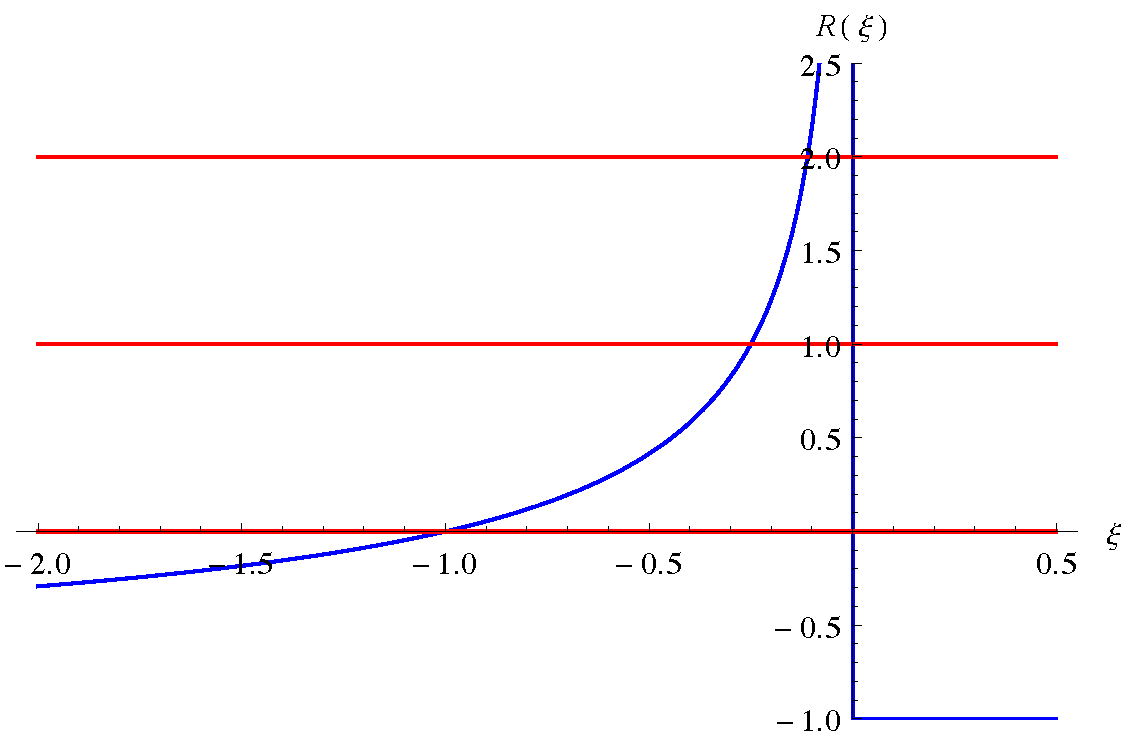
\includegraphics[scale=0.6]{Plots/ReNR.pdf}
\caption[Real part of the Regge trajectory function for the instantaneous scalar exchange model]{Real part of $R$ as a function of $\xi \equiv E / E_{R}$. The red lines correspond to $R = 0, 1, 2$. We have used $Z_{a} Z_{b} = -1$.}
\label{ReNRFig}
\end{figure}